% ======================================================================
% 第5章 提案手法
% ======================================================================

\section{概要}
本章では，第4章で述べた課題を解決するために構築した，提案手法の詳細なアルゴリズムと実装について述べる．
本研究では，PSOを経路制御に適用するための優先度ベースエンコーディング，制約条件を扱うための動的ペナルティ法，探索の停滞を打破する空間的lBestトポロジーとリスタート戦略，および計算時間を短縮するためのプロセス並列化を統合したシステムを実装した．

具体的な手順の説明に入る前に，本提案手法を構成する上で定めた3つの設計指針と，その採用理由について述べる．

\begin{enumerate}
    \item {優先度ベースエンコーディングの採用理由}:
    遺伝的アルゴリズム (GA) 等のメタヒューリスティクスを経路探索に適用する際，最大の問題となるのは「非実行可能解（ループや切断された経路）」の生成である．これらをペナルティ等で処理すると計算効率が著しく低下する．そこで本研究では，ノードへの優先度付けによる間接エンコーディングを採用することで，アルゴリズムが常に物理的に接続された有効なパスのみを探索対象とすることを保証し，無駄な探索を排除する．

    \item {空間的lBestトポロジーとリスタート戦略の導入理由}:
    標準的なPSO (gBestモデル) は収束が早いが，MCOPのような複雑な制約空間では局所解に陥りやすい．そこで，多様性を維持する空間的lBestトポロジーに加え，探索の停滞を検知して強制的に再探索を行うリスタート戦略を導入する．これにより，厳しい制約条件下であっても，単一の局所解に留まることなく，実行可能解を発見できるロバスト性を確保する．

    \item {並列化による計算効率の向上}:
    リスタート戦略は探索回数を増やすため，計算コストが増大する懸念がある．リアルタイム制御を実現するためには，このオーバーヘッドを解消する必要がある．そこで，粒子ごとの独立性が高いPSOの特性を活かし，評価プロセスを並列化することで，計算時間の短縮を図る．
\end{enumerate}

次節より，これらの指針に基づいた各要素技術の詳細について述べる．

\section{優先度ベースエンコーディング}
PSOは連続値ベクトルを扱う最適化手法であるため，これを離散的な構造を持つ経路探索問題に適用するには，粒子の位置情報を具体的な経路へ変換（デコード）する仕組みが必要となる．
本研究では，経路のエッジを直接最適化するのではなく，各ノードに割り当てられた実数値を選択優先度とみなして経路を構築する間接エンコーディング (Indirect Encoding) を採用した．
本手法における経路構築の概念図を図\ref{fig:encoding_concept}に示す．

\begin{figure}[tb]
  \centering
  \includegraphics[width=0.95\linewidth]{images/pathencoding.pdf}
  \caption{優先度ベースエンコーディングによる経路構築の概念図}
  \label{fig:encoding_concept}
\end{figure}

ネットワークのノード数を $N$ とするとき，各粒子 $i$ は $N$ 次元の位置ベクトル $\boldsymbol{x}_i = (x_{i,0}, x_{i,1}, \dots, x_{i,N-1})$ を持つ．
具体的な経路構築の手順は以下の通りである．なお，図\ref{fig:encoding_concept}における $k$ は探索のステップ数を，$V_p[k]$ はそのステップで選択されたノードを表している．

\begin{enumerate}
  \item 初期化 ($k=0$): 始点ノード $s$（図中の src）を現在のノード $u$ とする．
  \item 候補の作成: $u$ の隣接ノード集合 $Adj(u)$ を取得する．この際，ループを防ぐため，既に経路に含まれているノード（訪問済みノード）の優先度を一時的に十分小さな値（$-\infty$）に置き換え，選択候補から実質的に除外する．
  \item 次ホップの選択: 候補集合の中で，粒子ベクトル内の対応する値（優先度） $x_{i,v}$ が最大であるノード $v_{next}$ を次ホップとして選択する．
  \begin{equation}
    v_{next} = \argmax_{v \in Adj(u)} x'_{i,v}
  \end{equation}
  ここで，$x'_{i,v}$ は訪問済みノードの優先度がマスクされた後の値である．
  
  \item 経路の更新と終了判定: 選択された $v_{next}$ を経路リスト $V_p$ の $k$ 番目の要素として追加し，現在のノード $u$ を $v_{next}$ に更新する．
  終点 $d$（図中の dst）に到達するまで手順2-4を繰り返す．
\end{enumerate}

本手法の利点は，単純な大小比較のみで経路が決定するため計算コストが低い点（計算量はノード数 $N$ に対して $O(N)$）と，訪問済みノードを動的に除外することで閉路のない単純パス（Simple Path）が必ず生成される点にある．
なお，隣接ノードが全て訪問済みとなり，終点へ到達できずに行き止まり（Dead-end）となった場合は，その経路を無効解 (Invalid Solution) として扱い，適応度に大きなペナルティを与えることで次世代において淘汰させる．

\section{適応度関数と動的ペナルティ}
本研究の目的は，遅延，パケット損失率，信頼性の制約を満たしつつ，ボトルネック帯域幅を最大化することである．
これを実現するため，以下の適応度関数 $Fitness(\boldsymbol{x}_i)$ を設計した．

\begin{equation}
 Fitness(\boldsymbol{x}_i) = B(P) - \left( P_d \cdot \Delta D + P_l \cdot \Delta L + P_r \cdot \Delta R \right)
\end{equation}

ここで，$B(P)$ は構築された経路のボトルネック帯域幅である．
$\Delta D, \Delta L, \Delta R$ はそれぞれ遅延，損失，信頼性制約に対する違反量であり，違反がない場合は0となる．
$P_d, P_l, P_r$ はそれぞれの制約に対するペナルティ係数である．

また，探索の初期段階では実行可能領域への収束を促し，終盤では最適解の精度を高めるため，これらのペナルティ係数を世代数 $t$ に応じて線形に増加させる動的パラメータ調整を導入している．

\section{空間的lBestトポロジーとリスタート戦略}
本提案手法では，探索能力を向上させるために，空間的lBestトポロジーとリスタート戦略という2つの機構を導入している．

まず，トポロジー構造について述べる．
標準的なgBestモデルは収束が早いが局所解に陥りやすい．そこで本実装では，探索空間上でのユークリッド距離に基づく空間的lBest (Spatial lBest) トポロジーを採用した．
各粒子は，自身と距離が近い $k$ 個（本実験では $k=5$）の近傍粒子を特定し，その中での最良解 $lBest$ に引き寄せられる．
これにより，群れが複数のサブグループに分かれて探索を行う効果が生まれ，多様性が維持される．

さらに，この多様性維持に加え，探索の停滞（Stagnation）を検知し，局所解から脱出するための仕組みとしてリスタート戦略を実装した．
具体的には，実行可能解としての最大ボトルネック帯域 $gBest\_feasible\_bn$ が一定期間（20世代）更新されなかった場合，停滞と判断する．
停滞時は，現在の最良個体（エリート）1体を次世代に継承しつつ，残りの全粒子の位置と速度をランダムに再初期化する．これをExplosion（爆発）と呼ぶ．
この機構により，探索が局所解に捕らわれた場合でも，強制的に探索範囲を広げることで大域的最適解を発見できる可能性を高めている．

\section{並列化実装}
PSOの計算負荷の大部分は，粒子ごとの経路生成（PathEncode）と適応度評価に集中している．
本研究では，Pythonの `multiprocessing` モジュールを用いた同期型マスター・ワーカーモデルによる並列化を行った．
提案手法における並列処理の構造を図\ref{fig:parallel_model}に示す．

\begin{figure}[tb]
  \centering
  % PDFに変換した図を使用することを推奨します
  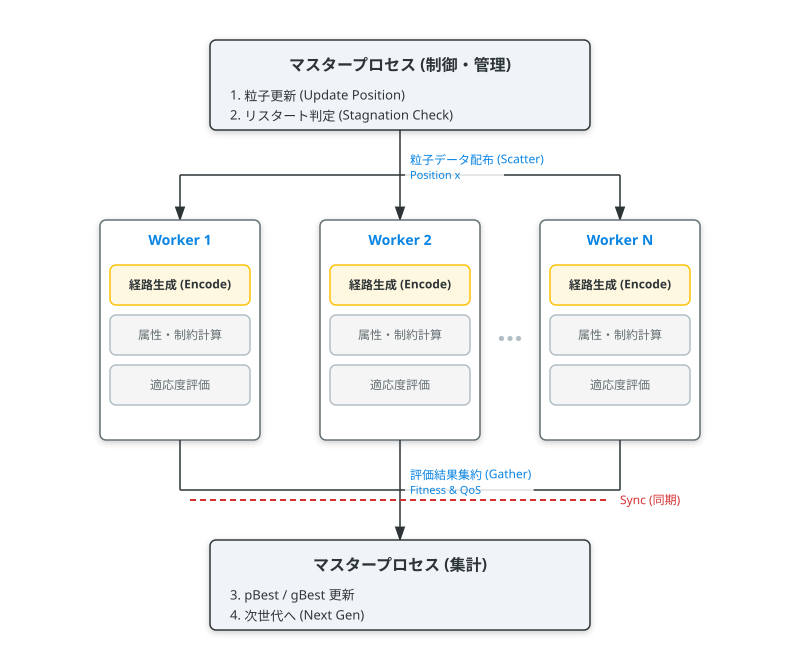
\includegraphics[width=0.95\linewidth]{images/parallel_model_final_v3.pdf}
  \caption{同期型マスター・ワーカーモデルによる提案手法の並列処理構造}
  \label{fig:parallel_model}
\end{figure}

本モデルは，制御・管理を行うマスタープロセスと，計算を行う複数のワーカプロセスから構成される．図\ref{fig:parallel_model}に示すように，処理の流れは以下の通りである．

\begin{enumerate}
    \item データ配布 (Scatter): マスタープロセスは，更新された各粒子の位置ベクトル $\boldsymbol{x}_i$ を各ワーカへ配布する（図中矢印：粒子データ配布）．
    \item 並列計算: 各ワーカは受け取った位置情報に基づき，以下の処理を順次実行する．
    \begin{itemize}
        \item 経路生成 (Encode): 図\ref{fig:encoding_concept}で示した優先度ベースエンコーディングにより経路を構築する．
        \item 属性・制約計算: 構築された経路のボトルネック帯域や遅延などのQoS属性値を計算する．
        \item 適応度評価: 制約違反量とペナルティを含めた適応度 $Fitness_i$ を算出する．
    \end{itemize}
    \item 結果集約 (Gather): 全ワーカの計算が完了するのを同期バリア (Sync Barrier) で待機した後，マスタープロセスは評価結果を集約する（図中矢印：評価結果集約）．
    \item 更新: 集約された結果に基づき，マスタープロセスが $pBest$ および $gBest$ の更新を行い，次世代の粒子位置を決定する．
\end{enumerate}

この同期型並列モデルにより，評価計算の負荷をコア数に応じて分散させ，特にノード数が増大した際のシミュレーション時間を大幅に短縮している．

\section{アルゴリズム全体の手順}
提案手法の全体的な処理フローを図\ref{fig:flowchart}に示す．
本アルゴリズムは，初期化の後，最大反復回数に達するまで並列評価，リスタート判定，速度・位置更新を繰り返す．

\begin{figure}[tb]
  \centering
  
\includegraphics[width=0.8\linewidth]{images/flowchart_restart_pso.pdf}
  \caption{提案手法（Restart PSO）の処理フローチャート}
  \label{fig:flowchart}
\end{figure}

Algorithm \ref{alg:proposed_method} に詳細な擬似コードを示す．

\begin{algorithm}[H]
\caption{リスタート戦略を用いた並列PSO (Proposed Method)}
\label{alg:proposed_method}
\begin{algorithmic}[1]
\Require グラフ $G$, 始点 $s$, 終点 $d$, 制約条件 $C$, 粒子数 $N$, 最大世代数 $T_{max}$
\Ensure 最良実行可能経路 $P_{best}$
\State 粒子位置 $\boldsymbol{X}$ と速度 $\boldsymbol{V}$ をランダムに初期化
\State $pBest$, $gBest$, $stagnation\_counter \leftarrow 0$ を初期化
\For{$t = 1$ to $T_{max}$}
    \State 動的ペナルティ係数 $P_d, P_l, P_r$ を更新
    \State \textbf{並列実行 (ワーカプロセスへ分散):}
    \For{各粒子 $i \in \{1, \dots, N\}$}
        \State $Path_i \leftarrow \text{優先度ベースエンコーディング}(\boldsymbol{x}_i, G, s, d)$
        \State 経路属性（帯域 $B_i$, 遅延 $D_i$, 損失 $L_i$, 信頼性 $R_i$）を計算
        \State $Fitness_i \leftarrow \text{適応度計算}(Path_i, C, P_d, P_l, P_r)$
    \EndFor
    \State 全粒子の $pBest_i$ を更新
    \State $gBest$ および 最良ボトルネック帯域 ($Best\_Feasible\_BN$) を更新
    \If{$Best\_Feasible\_BN$ が改善されない}
        \State $stagnation\_counter \leftarrow stagnation\_counter + 1$
    \Else
        \State $stagnation\_counter \leftarrow 0$
    \EndIf
    \If{$stagnation\_counter \ge Threshold$} \Comment{リスタート戦略 (Explosion)}
        \State 現在の $gBest$ (エリート) を保持
        \State 他の粒子の位置 $\boldsymbol{X}$ と速度 $\boldsymbol{V}$ をランダムに再初期化
        \State $stagnation\_counter \leftarrow 0$
    \EndIf
    \State 空間的近傍を計算し $lBest$ を決定
    \State 速度更新式および位置更新式を用いて $\boldsymbol{V}$ と $\boldsymbol{X}$ を更新
\EndFor
\State \Return 最終的な $gBest$ から構築された経路
\end{algorithmic}
\end{algorithm}

Algorithm \ref{alg:proposed_method} に示した提案手法の各ステップについて詳述する．

\paragraph{初期化 (Lines 1-2)}
まず，探索空間内において $N$ 個の粒子の位置ベクトル $\boldsymbol{X}$ と速度ベクトル $\boldsymbol{V}$ を一様乱数を用いて初期化する．
また，個体最良解 $pBest$ および大域最良解 $gBest$ を初期設定し，停滞検知用のカウンタ $stagnation\_counter$ を0にリセットする．

\paragraph{並列評価フェーズ (Lines 4-10)}
各世代において，まず制約条件に対する動的ペナルティ係数を更新する．
続いて，前述の並列モデル（図\ref{fig:parallel_model}）に従い，評価プロセスを複数のワーカプロセスに分散させて並列実行する．
各ワーカでは，粒子の位置ベクトルを受け取り，優先度ベースエンコーディングを用いて経路 $Path_i$ を構築する．
構築された経路に対し，ボトルネック帯域や遅延などの属性値を計算し，これらに基づいて適応度 $Fitness_i$ を算出する．

\paragraph{最良解の更新と停滞検知 (Lines 11-17)}
全粒子の評価が完了した後，$pBest$ および $gBest$ の更新を行う．
この際，制約条件を満たす実行可能解（Feasible Solution）の中で，最も高いボトルネック帯域を持つ解が見つかったかを判定する．
もし最良解が更新されなかった場合，停滞カウンタをインクリメントし，更新された場合はカウンタをリセットする．

\paragraph{リスタート戦略 (Lines 18-22)}
停滞カウンタが所定の閾値（本実験では20世代）に達した場合，探索が局所解に陥ったと判断し，リスタート戦略（Explosion）を発動する．
ここでは，これまでの探索で得られた最良の情報である $gBest$ を持つエリート粒子1体のみを次世代に残し，それ以外の全粒子の位置と速度をランダムに再初期化する．
これにより，探索空間の多様性を強制的に回復させる．

\paragraph{粒子の移動 (Lines 23-24)}
最後に，各粒子について空間的な近傍関係（ユークリッド距離に基づく近傍）から $lBest$ を決定し，PSOの基本式に従って次世代の速度と位置を更新する．
このサイクルを最大世代数 $T_{max}$ に達するまで繰り返すことで，最適経路を探索する．